%%=====================================================================
%% FUNDAMENTAÇÃO TEÓRICA (TCC, cap. 2): motor, hélice, SMO
%%=====================================================================
\secaoudesc{Fundamentação teórica}

\begin{frame}{Modelo do motor BLDC}
  \begin{columns}[c]
    \begin{column}{0.45\textwidth}
      \centering
      \tikzfig{1}{0.62}{motor_estrela}
    \end{column}
    \begin{column}{0.55\textwidth}
      \[ v_{k} = R\,i_k + L\,\frac{di_k}{dt} + e_k,
         \qquad e_k = k_e\,\omega_m\,f_k(\theta_e) \]
      \[ T_e = \frac{e_a i_a + e_b i_b + e_c i_c}{\omega_m} \]
      \[ J\,\frac{d\omega_m}{dt} = T_e - B\,\omega_m - T_L \]
      \begin{itemize}
        \small
        \item Transformada de Clarke: $abc \rightarrow \alpha\beta$
        \item A força contraeletromotriz (FEM) carrega a rotação e o ângulo
      \end{itemize}
    \end{column}
  \end{columns}
  \fonte[Autor (2026); Krishnan (2017); Clarke (1943)]
\end{frame}

\begin{frame}{Conjugado da hélice}
  \[ Q = C_Q\,\rho\,n^2 D^5, \qquad C_Q = \frac{C_P}{2\pi} \]
  \centering
  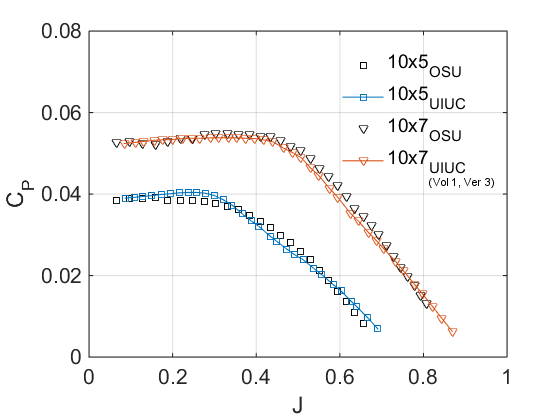
\includegraphics[height=0.62\textheight]{Revisao/Selig_propeller_data_cp.png}
  \fonte[McCrink e Gregory (2015); Selig (2026)]
\end{frame}

\begin{frame}{Ponto de operação}
  \begin{columns}[c]
    \begin{column}{0.36\textwidth}
      \begin{itemize}
        \item Torque da hélice cresce com $n^2$
        \item Cruzamento com a curva do motor define rotação, corrente e tração
        \item Hélices de referência: APC 15x6E e 17x10E
      \end{itemize}
    \end{column}
    \begin{column}{0.64\textwidth}
      \centering
      \tikzfig{1}{0.7}{helice_ponto_op}
      \fonte[Autor (2026); Brandt et al.\ (2015)]
    \end{column}
  \end{columns}
\end{frame}

\begin{frame}{Observador por modos deslizantes (SMO)}
  \centering
  \tikzfig{1}{0.62}{smo_generico}
  \begin{itemize}
    \small
    \item Estima as correntes e força o erro a zero com um termo chaveado
    \item O sinal de chaveamento, filtrado, é a FEM: dela saem rotação e ângulo
  \end{itemize}
  \fonte[Adaptado de Utkin (1992); Slotine e Li (1991)]
\end{frame}
